\documentclass[%
 onecolumn,notitlepage,
%superscriptaddress,
%groupedaddress,
%unsortedaddress,
%runinaddress,
%frontmatterverbose, 
%preprint,
%showpacs,preprintnumbers,
%nofootinbib,
%nobibnotes,
%bibnotes,
 amsmath,amssymb,
 aps,
 longbibliography
%prl,
%pra,
%prb,
%rmp,
%prstab,
%prstper,
%floatfix,
]{revtex4-1}
\usepackage{float}
\usepackage{graphicx}% Include figure files
\usepackage{epstopdf}
\usepackage{dcolumn}% Align table columns on decimal point
\usepackage{bm}% bold math
\def\dbar{{\mathchar'26\mkern-12mu \mathrm{d}}} 
\usepackage{amsmath}
\usepackage{physics}

\makeatletter
\newcommand{\rmnum}[1]{\romannumeral #1}
\newcommand{\Rmnum}[1]{\expandafter\@slowromancap\romannumeral #1@}
\makeatother

\usepackage{fancyhdr}

\pagestyle{fancy}
\fancyhf{}
%\fancyhead[LE,RO]{Share\LaTeX}
\fancyhead[RE,LO]{Neutron Stars}
\fancyfoot[CE,CO]{\leftmark}
\fancyfoot[LE,RO]{\thepage}


\fancypagestyle{firstpage}{%
  \fancyhf{}
  \fancyhead[LE,RO]{Second Year Theory Computing Project}
\fancyhead[RE,LO]{Neutron Stars}
\fancyfoot[CE,CO]{\leftmark}
\fancyfoot[LE,RO]{\thepage}
}
 
\renewcommand{\headrulewidth}{1.5pt}
\renewcommand{\footrulewidth}{0pt}
\newcommand{\squeezeup}{\vspace{-2.5mm}}

  
%\usepackage{hyperref}% add hypertext capabilities
%\usepackage[mathlines]{lineno}% Enable numbering of text and display math
%\linenumbers\relax % Commence numbering lines

%\usepackage[showframe,%Uncomment any one of the following lines to test 
%%scale=0.7, marginratio={1:1, 2:3}, ignoreall,% default settings
%%text={7in,10in},centering,
%%margin=1.5in,
%%total={6.5in,8.75in}, top=1.2in, left=0.9in, includefoot,
%%height=10in,a5paper,hmargin={3cm,0.8in},
%]{geometry}

\begin{document}

\section{Conventional accelerators}\vspace{-8pt}
An estimated 30 000 particle accelerators are currently in operation worldwide, 
%forming an integral part of many areas of science and industry.
providing beams of high-energy particles for science and industry. 
For instance, monoenergetic electron bunches allows for the generation of high-quality X-ray pulses through the use of undulators; a technique by which high-energy electron bunches are rapidly oscillated back-and-forth perpendicular to their direction of propagation. This oscillatory motion can generate highly coherent synchrotron radiation in the X-ray spectrum using  ultra-relativistic electrons , which can be used in medicine for advanced tissue diagnostics  (something tomography) (add length) . Operating at higher energies, the 1.7 km long European free electron laser (XFEL) facility in Hamburg, Germany, uses 17.5 GeV electron bunches to generate ultra short, extremely brilliant X-ray pulses which are used for fundamental research into the structure proteins, molecules..and even create movies of molecular motion \cite{xfel}. Probing even smaller length scales takes us into the realm of high-energy physics, where the size of the accelerators grows accordingly. From the ... long SLAC Linear Colider (SLC) at Fermilab to the Large Electron Positron colider (LEP) which accelerated electrons and positrons up to 100 GeV and now named the LHC accelerates protons to 14TeV, the fine details of the smallest constituents of our theories is being explored through tests of the standard model. Even more energetic accelerators, such as the International Linear Collider (ILC) will push the particle energies even higher. However, as energy increases, the size of the accelerator increase as well. \\
\indent The reason for this increase stems from the method by which particles are accelerated. High-energy particle accelerators rely on resonant radiofrequency (RF) cavities. These are evacuated cavities which the particle beam passes through. The design and operation of these cavities are carefully engineered so as to set up an oscillating electric potential which acts to accelerate and squeeze the particle bunches together. The current RF cavities at the LHC privde an accelerating field of 5MV/m, such that the energy gain per meter is 5MeV. Hence, to reach TeV energies the protons at the LHC needs to pass through tens of millions RF cavities, which clearly necessitates a circular accelerator. The large size of the LHC then comes from the fact that the bending of the particles around the circular accelerator is limit by the magnetic field strength and the emission of synchrotron radiation.  [Add how much more energy LEP would have required to find the higgs]. Even if one used a combination of circular accellerators feed into a linear accelerator to avoid synchrotron energy loss, as in the proposed ILC, the size would still need to be large given that the maximum electric acceleration field in an RF cavity is $~$ 100MV/m, beyond which point....rf breakdown (seperation of ions and electrons). Clearly, even if the particle physics community is granted ever increasing particle accelerators, as the demand for GeV particle accelerators grows in medicine, industry and fundamental research, the size and cost of accelerators is and will continue to be a limit factor to future progress if no other means of acceleration is possible.\vspace{-8pt}
\section{Plasma wakefield accelerators}\vspace{-8pt}
Several novel accelerators techniques exists in various stages of development. The most widespread of these is based on the phenomena of \textit{plasma wakefield acceleration}. Driving a relativistic particle beam or a high intensity laser pulses through a preformed plasma can excite waves in the plasma with phase velocities equal to the group velocity of the particle or laser driver [Plasma Wakefield Acceleration for Ultrahigh-Energy Cosmic Rays]. The waves, or "wakefields", are large-amplitude oscillations of the plasma-electron density behind the driver which are able to support accelerating fields of hundrends of GV/m; thousands of times higher than conventional RF cavities. By injecting an electron, or positron, bunch behind the driver one can then achieve constant acceleration by effectively letting the particle bunch surf the plasma-electron wave. In this manner, huge energy gains can be achieved over relatively short propgation distances if a sufficiently powerful driver is avilable. In fact, in this form of plasma enabled acceleration was proposed in 1979 by Tajima and Dawson [], not only as a viable terrestrial particle accelerator but also as a generation mechanism of ultra-high-energy cosmic rays in the plasma rich environment around newly formed pulsars. At this point in time the lack of sufficiently high intensity lasers was a limit factor in exploring these ideas experimentally. The invention of the chirped-pulse amplification techniques for lasers in the 1980s by Strickland and Mourou \footnote{2018 Nobel prize }[] gave researchers access to ultrashort high-intensity laser pulses. This opened up the possibility of laser driven plasma wakefield acceleration and several experiments followed [Kieran's thesis].\textbf{lwfa, then pwfa, FACET,DESY,AWAKE}\\ 
These experiments are paving the way towards compact high-energy particle accelerators at GeV energies with great promise to science and industry. One can also imagine a future in which plasma wakefield accelerators are used in high-energy physics, perhaps in conjugation with conventional accelerators as a pre-accelerator [?] or as an energy booster. Even though the latter is probably decades away, both GeV and TeV accelerators might still be able to benefit from plasma wakefield phenomena. Regardless of the means of acceleration, be it larger conventional accelerators or smaller plasma wakefield accelerators, the ultra-relativistic beams produced will need to be dealt with. The current approach for both small and large accelerators is to dump the energy of the beam. \vspace{-8pt}
\section{Beam dumps}\vspace{-8pt}
%Small accelerator dumps,

When in operation, the 100 GeV electron and positron beams at the LEP at CERN were expanded, to decrease the intensity, and directed into a 2 m long, 40 cm in diameter, aluminium alloy block in order to be brought to a stop \cite{LEP_dump}. The proposed water-based beam dump for the ILC \cite{Satyamurthy2012}, which is to operate at 500 GeV, is significantly different to its lower energy predecessor at LEP. The increased energy and intensity of the ILC beam makes the extraction of its energy from a solid material beam dumps exceedingly difficult because of the limitations imposed by thermal conduction [Design of an 18 MW]. By using a ... m3 tank of water the ILC beam energy can be deposited and removed using a pumping system. The high intensity beams however lead to water temperatures in excess of 150C, resulting in ...(catalysis?) of water into hydrogen and oxygen gas. This necessitates a safe and efficient way to remove and store these gases. Furthermore, the beam interaction with the water molecules will create the radioactive nuclei Be7 and..., this requires a waste-water storage tank which will need to be treated. The tank itself will also suffer radiation damages, specifically the window through which the beam enters the vessel. A report by ...et al. \cite{Satyamurthy2012} estimates that this window will need to be replaced at ... intervals. Due to the induced radioactivity this will have to be done remotely, using robotic technology. Although this technology is widely available in the nuclear industry this whole beam dump is a large and costly affair for the ILC and any future HEP accelerators. \\
%The situation for its predecessor the LHC is similar, however the much larger energy carried by the protons requires a correspondingly larger beam dump. In this case, the 7 TeV proton beams are expanded and directed into a cylinder of graphite composite, 8 m long and 1 meter in diameter, which gets heated to 700\degree C upon impact and therefore contained in a water-cooled steel cylinder. This in turn, is encased in 750 tonnes of concrete and iron shielding [The LHC Beam Dumps website]. 
An alternative approach utilizes the huge acceleration gradients from PWFA. This idea was proposed in 2010 by Wu et al. \cite{Wu2010}. They showed through simulations that a 500 MeV electron bunch, under certain conditions, could loose up to 70\% of its energy by propagating a few millimetres through a dense plasma, a so-called passive plasma beam dump. Full energy depletion was prevented by decelerated particles in the bunch reaching non-relativistic speeds and falling behind the main bunch, at which point they where picked up by the accelerating portion of the field and reaccelreated to realtivisitic speeds, the bunch energy is said to have saturated. It was further found that the decelerating field was independent of the initial bunch energy, such that the distance to saturation scaled linearly with bunch energy, such that a 100 GeV bunch would require $~20$ cm to loose 70\% of its energy. To avoid re-acceleration they stragetically placed thin aerogel foils in the plasma to stop the low energy particles before re-acceleration. Using this improved the energy depletion up to 90\% for 500 MeV bunch.  Due to the finite response time of the plasma, the head of the bunch displaces the plasma electrons and sets up the wakefield but due not experience the huge decelerating gradients further back. For this reason the head of the bunch looses essentially no energy, known as "energy chirp", as can be seen in the original plots from the paper by Wu et al.  in figure \ref{Wu}. For a 500 MeV or a few GeV bunch this might not be a major issue since smaller conventional beam dumps could be used to dump this remaining energy. For energies of 100s of GeV however this energy chirp could still pose an issue in terms of radioactivity of materials. Furthermore, it is not clear how the proposed intermediate foils would de-gradate and behave under the extereme conditions of high-energy beams.\\
\begin{figure}
\centering
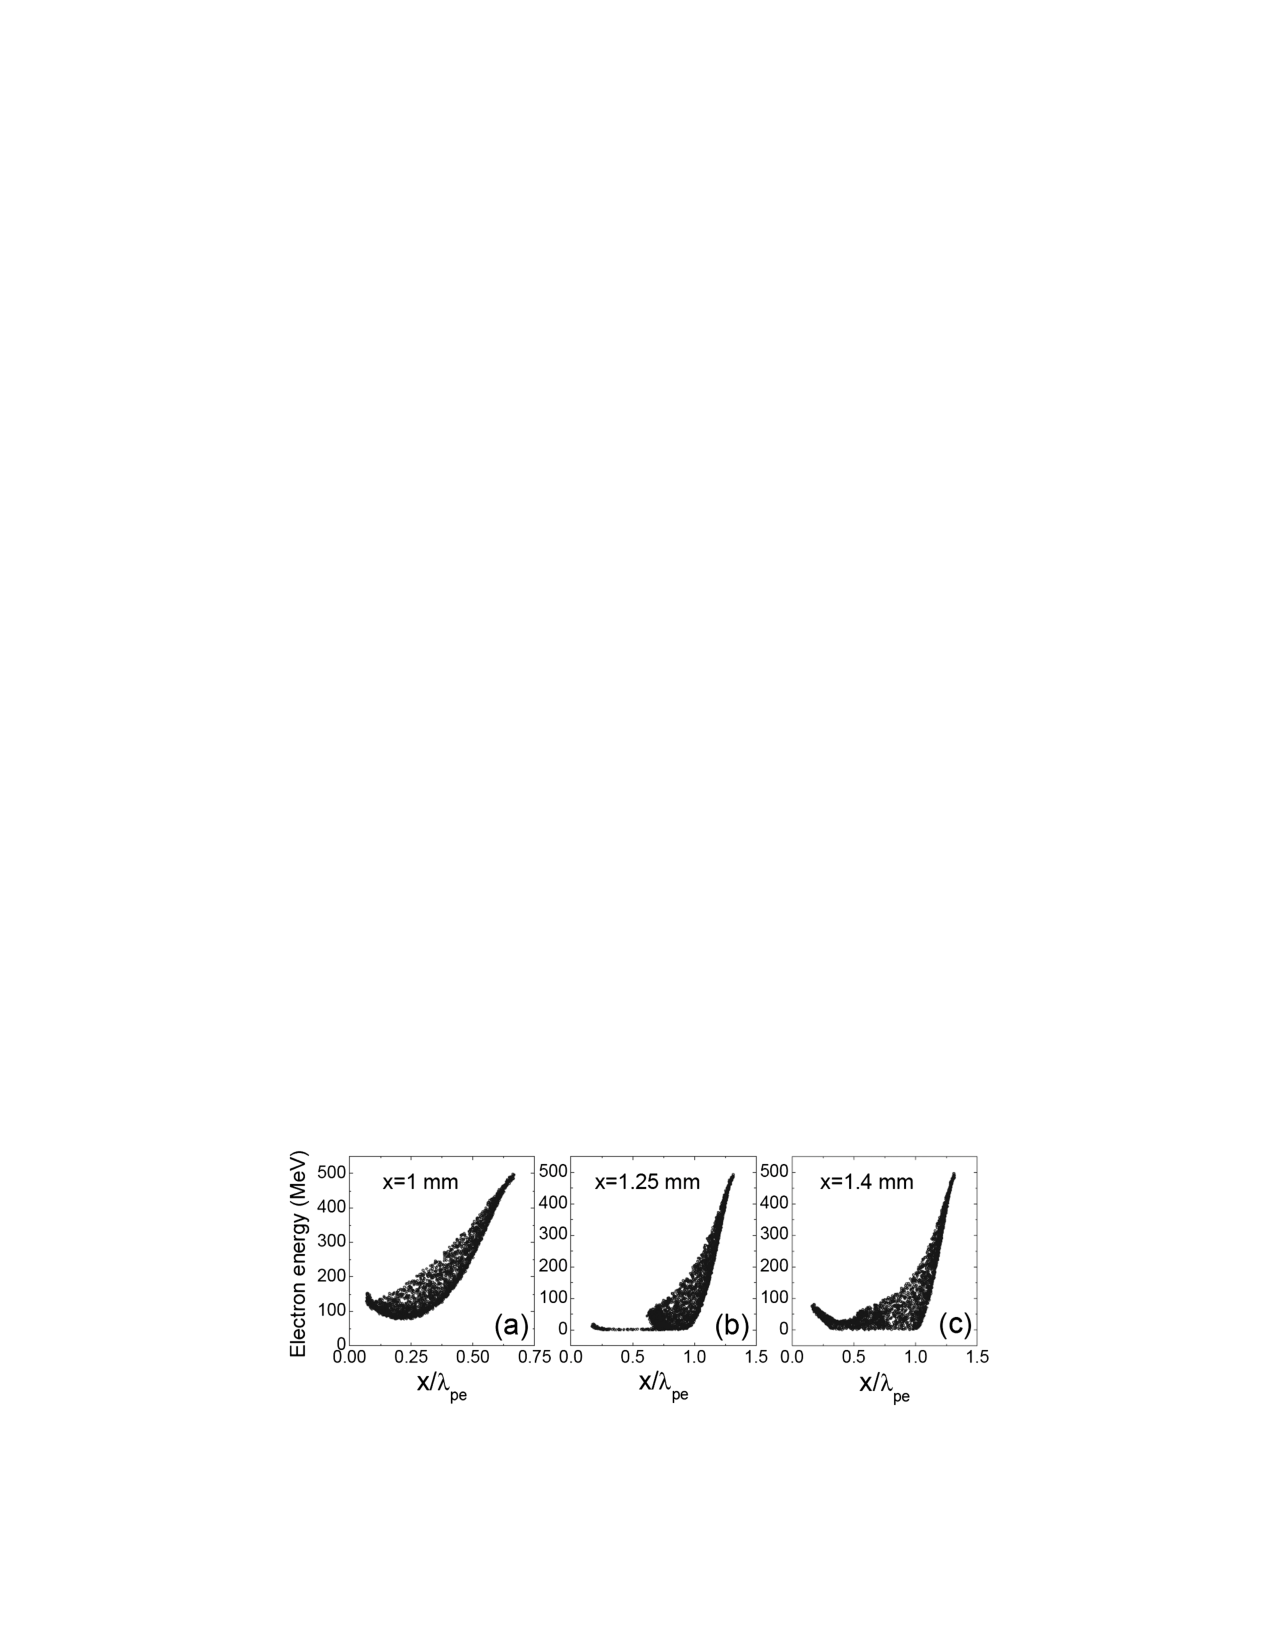
\includegraphics[width=0.9\textwidth]{Wu_energy_uniform.pdf}
\caption{}
\label{Wu}
\end{figure}
To address the energy chirp Bonatto et. al \cite{Bonatto2015} propsed the so-called active beam dump, whereby a laser is driven through the plasma in front of the bunch that is to be decelerated. By carefully positioning the laser in relation to a 1 GeV bunch it was shown that the energy in the head of the bunch could be significantly reduced, resulting in a total energy depletion up to 95\%. It is however difficult to apply this method to higher energy bunches since the dispersion of the laser in the plasma prevents laser propagation over long distances. \\
Finally, Hanahoe et al. \cite{Hanahoe2017} proposed the use of varying plasma density instead of foils as an alternative way to prevent reaccelration. Linear or quadratically increasing plasma densities were shown to achieve comparable reduction of the reaccelrated particles as the foils used by Wu et al.  It is however unclear whether such plasma density profiles can be set up and sustained reliably in an experimental setting. \\
With several proposed plasma beam dump techniques in place this project endeavours to merge the passive and active approaches in what we call a hybrid plasma beam dump, with the goal of achieving a full energy depletion of the bunch. In addition, simulations will also be carried out for a recently approved plasma beam dump experiment at the FLASHForward facility at DESY in Germany. This will be the first dedicated plasma beam dump experiment of its kind and will be capable of testing both the passive and active approaches described above. 
\section{Outline of report}
This intermediate report details the initial phase of a full-year project on plasma wakefield deceleration and is written in partial fulfilment of the requirements for the degree of Master in Physics. As such, it does not attempt to cover the full scope of the work and research conducted in the first half of this project, but rather aims to provide and introduction to the field, establish the theoretical background and construct the computational framework necessary to perform the intended research. Having lain the groundwork for the project in this report, the the final-year report will reap the rewards of this work by presenting the full results and outcome of the project.\\
The theory behind plasma wakefield acceleration and plasma beam dumps is covered in section 2. The simulation framework is detailed in section 3, followed by simulation tests and preliminary results in section 4. We conclude this report by summarising the work that has been presented and looking ahead at the work that is to be carried out in the second half of this project.
\\
\\
Superconduction RF (https://www.youtube.com/watch?v=HqrSb36QYVk)
\end{document}
